%%
%% Capítulo 2: Regras gerais de estilo
%%

\mychapter{Fundamentação Teórica}
\label{Cap:Teoria}

Neste capítulo serão apresentados os conceitos básicos relacionados ao \textit{framework Flutter}, assim como a linguagem de programação Dart, a biblioteca MobX e o \textit{wrapper} Provider, utilizados para o desenvolvimento desta aplicação.

Também serão discutidas as principais ideias relacionadas à Programação Orientada a Objeto (POO), aos bancos de dados relacionais e, por fim, alguns conceitos relacionados às boas práticas da programação no quesito de arquitetura de sistemas e os princípios SOLID.

\section{Dart}
\label{cap2:Sec:Dart}

Nessa seção, busca-se apresentar os conceitos básicos da linguagem Dart, utilizada para o desenvolvimento do \textit{framework} Flutter. O foco agora é mostrar as características que fizeram com que a linguagem Dart foi escolhida para ser a linguagem de programação do \textit{framework} Flutter.

\subsection{Introdução}
\label{cap2:SubSec:Introducao}

Dart é uma linguagem de programação criada pela Google em 2011, com o objetivo de ser utilizada, inicialmente, para o desenvolvimento de aplicações web, mas que tem como objetivo atual ser executada em qualquer plataforma.
% ref: http://googlecode.blogspot.com/2011/10/dart-language-for-structured-web.html 04/11/2022
% ref: https://dart.dev/overview#platform:~:text=Learning%20Dart-,Dart,-is%20a%20client 04/11/2022

A linguagem é orientada a objetos, fortemente tipada e compilada. Ela possui uma sintaxe similar às linguagens C, mas com algumas diferenças, como a utilização de palavras-chave como \textit{var} e \textit{final} para declarar variáveis e \textit{null} para representar a ausência de valor. A linguagem também se assemelha a outras comumente utilizadas no desenvolvimento de aplicações móveis, web e desktop, como Java, Kotlin, Swift e Typescript, por exemplo.
% ref: https://dart.dev/#:~:text=learn%2C%20with%20a-,familiar%20syntax,-Productive%20development 05/11/2022
% ref: https://dart.dev/guides/language/language-tour#important-concepts 05/11/2022


\subsection{Compilação}
\label{cap2:SubSec:Compilacao}
\textit{Dart} possui duas estratégias de compilação que são utilizadas em conjunto, mas em períodos diferentes do processo de desenvolvimento e de utilização da aplicação. Além disso, a linguagem utiliza-se de uma máquina virtual chamada \textit{Dart VM} para executar o código durante o desenvolvimento da aplicação ou traduz o código \textit{Dart} em \textit{JavaScript} para plataforma \textit{web}.
% ref: https://dart.dev/overview#platform 05/11/2022

Linguagens dinâmicas como JavaScript, às quais permitem ao desenvolvedor criar variáveis dinâmicas, ou seja, que podem mudam seus tipos em tempo de execução, utilizam a compilação \textit{Just-in-time (JIT)}. Esse tipo de compilação permite que o desenvolvimento se torne mais produtivo ao diminuir o tempo de espera entre uma mudança no código e a execução do mesmo para avaliar o resultado. Por outro lado, linguagens estáticas como C utilizam-se da estratégia de compilação \textit{Ahead-of-time (AOT)}. Dessa forma, todo o código deve ser compilado antes da execução do programa, o que torna o tempo de espera entre uma mudança no código e sua nova execução maior. Enquanto o \textit{JIT} tem vantagens sobre o \textit{AOT} em termos de produtividade, o \textit{AOT} tem vantagens em termos de performance, pois não há a necessidade de pausa na execução no código para análise ou compilação \textit{JIT}. Isso faz com que a aplicação seja inicializada e executada mais rapidamente. 
%  ref: https://hackernoon.com/why-flutter-uses-dart-dd635a054ebf 05/11/2022

% Colocar uma imagem aqui


No \textit{Dart}, a estratégia de compilação \textit{JIT} é utilizada no período de desenvolvimento da aplicação, enquanto a compilação \textit{AOT} é utilizada para a compilação final da aplicação. O código compilado é otimizado para a plataforma em que será executado. Por exemplo, o código compilado para dispositivos móveis é otimizado para a arquitetura \textit{ARM}, enquanto o código compilado para \textit{desktop} é otimizado para a arquitetura \texttt{x64}.
% ref: https://dart.dev/overview#platform 05/11/2022
% ref: https://dart.dev/ 01/11/2022

\begin{figure}[!ht]
  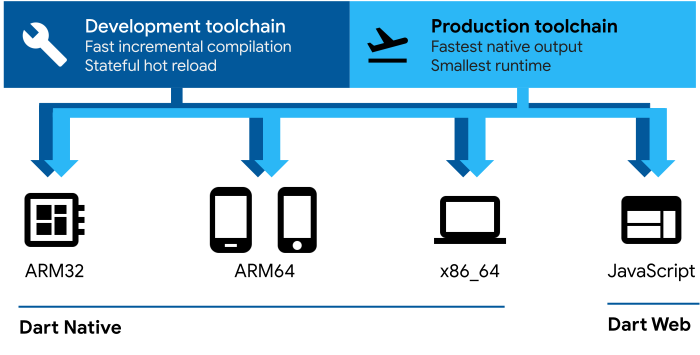
\includegraphics[width=1\textwidth, keepaspectratio=true]{figuras/cap2/2_1_2_dart-platforms.png}
  \centering
  \caption[Plataformas de compilação do Dart]{Plataformas de compilação do Dart \protect\cite{dart-platforms}}
  % \font{Site oficial da linguagem Dart}
  \label{fig:dart_plataforms}
\end{figure}
% \FloatBarrier

Outras características do \textit{Dart} levaram ao seu uso no \textit{Flutter}:

\begin{itemize}
  \item \textbf{ausência de troca de contexto} com a plataforma: como o código compilado é nativo e não possui análises ou novas compilações \textit{JIT}, não há a necessidade de troca de contexto entre a plataforma e a linguagem, o que torna a execução mais rápida;
  % ref: https://hackernoon.com/why-flutter-uses-dart-dd635a054ebf 05/11/2022
  \item \textbf{\textit{single-threaded}}: a preemptividade, isto é, o procedimento de interromper uma tarefa para a execução de outra \textit{thread}, utilizadas em linguagens como \textit{Java} ou \textit{Kotlin} não existe, pois o \textit{Dart} é \textit{single-threaded}, ou seja, não há compartilhamento de memória, nem a necessidade de gerenciamento de estado entre as \textit{threads}, o que evita a possibilidade de erros como condições de corrida ou \textit{deadlock}s;
  \item Uso de \textbf{\textit{isolates}}: todo o código em \textit{Dart} roda dentro de \textit{isolates}, o qual possui um uma única \textit{thread} e se comunica com outros \textit{isolates} por meio de mensagens. Mesmo ações assíncronas são gerenciadas com o uso de classes como \textit{Future} e \textit{Stream} ou com o uso de \textit{async/await}. Dessa forma, o \textit{Dart} é capaz de executar código assíncrono sem a necessidade de novas \textit{threads}. Em última instância, é possível criar um \textit{background isolate}, que será responsável por realizar algum tipo de tarefa em segundo plano, como por exemplo, a leitura ou escrita de um arquivo e devolver seu resultado ao \textit{main isolate} me forma de mensagem quando finalizado.
  % ref: https://dart.dev/guides/language/language-tour#isolates 05/11/2022
% ref: https://dart.dev/guides/language/concurrency#how-isolates-work 05/11/2022
  \item Esquema de \textbf{garbage collection} (GC): a linguagem \textit{Dart} utiliza um avançado esquema de coleta de lixo geracional e que se divide em duas fases. Esse algoritmo favorece a rápida criação e destruição de objetos, o que é comum em aplicações feitas com Flutter, que possui muitos objetos sendo alocados e desalocados, como por exemplo, os \textit{Stateless Widgets}.
  % ref: https://hackernoon.com/why-flutter-uses-dart-dd635a054ebf#:~:text=Allocation%20and%20garbage%20collection 05/11/2022
  % ref: https://medium.com/flutter/flutter-dont-fear-the-garbage-collector-d69b3ff1ca30
\end{itemize}



\section[\textit{Flutter}]{Flutter}
Busca-se apresentar, nesta seção, uma visão em alto nível do que é o \textit{framework Flutter}, sua arquitetura, as principais características da tecnologia e suas diferenças para as demais tecnologias no mercado.

O \textit{Flutter}, criado pela \textit{Google}, é desenvolvido em código aberto e visa possibilitar o desenvolvimento de aplicações \textit{Android}, \textit{Web}, \textit{Desktop} e de \textit{software} embarcado a partir de uma única base de código, compiladas nativamente. A aplicação é mantida não só pela empresa que a criou, mas também recebe novas atualizações e incorporações advindas da comunidade.
% ref: https://docs.flutter.dev/resources/faq#what-is-flutter 30/10/2022


\subsection{Arquitetura do \textit{framework}}
\label{cap2:SubSec:ArquiteturaFlutter}
A fazer.
% [A fazer] Falar sobre o hot reload e relacionar com o JIT do Dart VM (https://hackernoon.com/why-flutter-uses-dart-dd635a054ebf#:~:text=a%20game%20changer%E2%80%A6-,Stateful%20hot%C2%A0reload,-One%20of%20the e )
% [A revisar] O \textit{framework} é composto por três camadas principais: \textit{widgets}, \textit{rendering} e \textit{gestures}. A camada de \textit{widgets} é responsável por definir os elementos visuais da aplicação, enquanto a camada de \textit{rendering} é responsável por desenhar os elementos na tela. A camada de \textit{gestures} é responsável por capturar os eventos de interação do usuário com a aplicação, como toques na tela, movimentos do mouse, etc.
% ref: https://flutter.dev/docs/resources/architectural-overview 01/11/2022

\subsection{\textit{Widgets}}
\label{cap2:SubSec:Widgets}
O \textit{framework} recebe inspiração do React e, dessa forma, utiliza-se de \textit{widgets} (\ref{fig:nurse-widget-tree}) para compor os elementos visuais das aplicações, assim como os estados dos mesmos. % ref: https://docs.flutter.dev/development/ui/widgets-intro 01/11/2022
Estes \textit{widgets} devem ser responsáveis por gerir, com boa performance, a renderização dos elementos na tela, suas animações e também controlar as interações do usuário com a aplicação.
% ref.: Wenhao Wu: React Native vs Flutter, cross-platform mobile application frameworks: 2.2.3 Widget: Widgets do not only control and affect how the views behave, but also handle and respond to the user’s action. Thus, it is crucial that Widgets need to perform fast, including rendering and animating. 01/11/2022

\begin{figure}[ht!]
    	
  \centering
          \subfloat[Representação da árvore de \textit{widget}s]{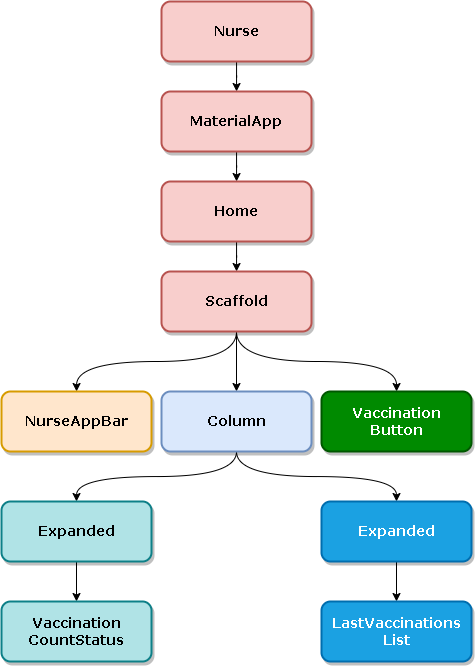
\includegraphics[width=0.45\columnwidth]{figuras/cap2/2_2_2_nurse-widget-tree.png}}
            \qquad
            \subfloat[Árvore apresentada pelo \textit{Flutter DevTools}]{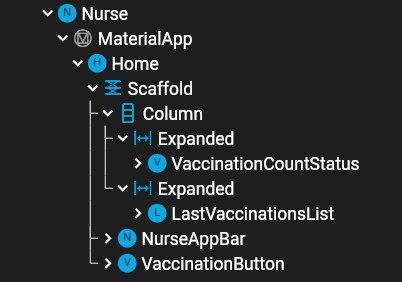
\includegraphics[width=0.45\columnwidth]{figuras/cap2/2_2_2_nurse-widget-tree-flutter-tool.png}}
    \caption[Estrutura simplificada de \textit{widgets} da aplicação \textit{Nurse}]{Estrutura simplificada de \textit{widgets} da aplicação \textit{Nurse}}
  % \fonte{Inserir autor aqui}
  
  \label{fig:nurse-widget-tree}
\end{figure}
% \FloatBarrier
  
Além disso, os \textit{Widgets} devem ser customizáveis e extensíveis, de forma que possam ser flexíveis em relação às suas propriedades e reuso. O Flutter possibilita isso ao trazer a responsabilidade de criação e renderização dos \textit{Widgets} da plataforma à qual está rodando para própria aplicação. Posteriormente, na seção \ref{cap2:Subsec:DiferencasTecnologias}, será apresentada uma breve explicação da diferença entre o tratamento de \textit{Widgets} feito pelo Flutter e por outras tecnologias, como o \textit{React Native}, \textit{WebViews} e aplicações escritas em Android ou iOS.
 % ref: https://hackernoon.com/whats-revolutionary-about-flutter-946915b09514


A seguir, serão apresentados os dois principais tipos de \textit{widgets} utilizados no desenvolvimento da aplicação, suas principais características e diferenças. São eles: \textit{Stateless Widgets} e \textit{Stateful Widgets}, que diferem entre si, essencialmente, pelo gerenciamento ou não de seu estado interno. % ref: https://docs.flutter.dev/development/ui/widgets-intro 01/11/2022

\subsubsection{Stateless Widgets}
\label{cap2:SubSubSec:StatelessWidgets}
Os \textit{stateless widgets} são \textit{widgets} que não possuem mudança estado, ou seja, não possuem propriedades que podem ser alteradas ao longo do tempo, como por exemplo, quando há uma animação ou um campo de texto ao qual um usuário possa interagir e, assim, só dependem das configurações definidas pelo próprio objeto e o contexto em que ele está inserido. Esses \textit{widgets} podem ser utilizados para representar elementos estáticos da interface, como textos, imagens, botões etc. A seguir, é apresentado um exemplo de um \textit{stateless widget} que representa um botão.
% https://api.flutter.dev/flutter/widgets/StatelessWidget-class.html 01/11/2022
% ref: https://www.youtube.com/watch?v=wE7khGHVkYY 06/11/2022

\begin{lstlisting}[caption={Exemplo de um \textit{stateless widget} que representa um botão.}, label={lst:stateless_widget}]
  class BotaoPrincipal extends StatelessWidget {
    final String texto;
  
    const BotaoPrincipal(Key? key, this.texto) : super(key: key);
  
    @override
    Widget build(BuildContext context) {
      return TextButton(
        onPressed: () => {print("Clicou no botao principal")},
        child: Text(texto),
      );
    }
  }
\end{lstlisting}

No código \ref{lst:stateless_widget} temos a \textbf{classe BotaoPrincipal} que estende um \textit{StatelessWidget} e possui um atributo \textbf{texto} que é passado como parâmetro para o construtor da classe e não pode ser modificado posteriormente (regra garantida pela palavra chave \textit{final} que antecede o tipo da variável). A classe possui um método \textbf{build} que retorna um \textit{widget} do tipo \textit{TextButton} que recebe como parâmetro uma função anônima que imprime uma mensagem no console e um \textit{widget} do tipo \textit{Text} que recebe como parâmetro o atributo \textbf{texto} da classe. No lugar da função de impressão da mensagem em tela poderia ser passado uma função que redireciona o usuário para outra tela, por exemplo.


% https://flutter.dev/docs/development/ui/widgets-intro#stateless-and-stateful-widgets
\subsubsection{Stateful Widgets}
\label{cap2:SubSubSec:StatefulWidgets}
% [A revisar]
Os \textit{stateful widgets} são \textit{widgets} que possuem mudança de estado, ou seja, possuem propriedades que podem ser alteradas ao longo do tempo, como por exemplo, quando há uma animação ou um campo de texto ao qual um usuário possa interagir e, assim, dependem não só das configurações definidas pelo próprio objeto e o contexto em que ele está inserido, mas também do estado interno do objeto. A seguir, é apresentado um exemplo de um \textit{stateful widget} que representa um campo de texto.
% ref: https://api.flutter.dev/flutter/widgets/StatefulWidget-class.html 07/11/2022

% [A revisar]
\begin{lstlisting}[caption={Exemplo de um \textit{stateful widget} que representa um campo de texto.}, label={lst:stateful_widget}]
  class CampoTexto extends StatefulWidget {
    final String texto;

    const CampoTexto({Key? key, required this.texto}) : super(key: key);

    @override
    State<CampoTexto> createState() => _CampoTextoState();
  }

  class _CampoTextoState extends State<CampoTexto> {
    String texto = "";

    @override
    Widget build(BuildContext context) {
      return TextField(
        onChanged: (value) {
          setState(() {
            texto = value;
          });
          print(texto);
        },
        decoration: InputDecoration(
          labelText: widget.texto,
          hintText: "Digite aqui",
        ),
      );
    }
  }
\end{lstlisting}

O \textit{stateful widget} é dividido em duas classes, ou em dois objetos distintos que se contemplam, como pode ser observado no código \ref{lst:stateful_widget}.
% ref: https://medium.com/flutter-community/widget-state-buildcontext-inheritedwidget-898d671b7956 07/11/2022
A primeira classe, a qual estende de \textit{StatefulWidgets} é imutável e também podem receber variáveis via construtor, mas que são finais, assim como as propriedades das classes do tipo \textit{StatelessWidget}'s. Para que hajam mudanças, um objeto do tipo \textit{State} é adicionado e este será responsável pelas mudanças que poderão ocorrer no ciclo de vida do \textit{StatefulWidget}.

A classe que estende \textit{State} (chamada \textbf{CampoTextoState} no exemplo), criada no momento em que a função \textit{StatefulWidget.createState()} é chamada, representa a informação lida pelo \textit{widget} e que pode ser alterada durante o tempo de vida do mesmo.
% ref: https://api.flutter.dev/flutter/widgets/StatefulWidget-class.html 07/11/2022
Além disso, o estado em si pode ter um ciclo de vida maior que o do seu próprio \textit{widget}, mantendo-se em memória mesmo quando este é reconstruído.
% ref: Sebastian Faust: Using Google´s Flutter Framework for the Development of a Large-Scale Reference Application: 3.4.2 Stateful Widgets 07/11/2022

O ciclo de vida de um \textit{State} engloba as seguintes etapas principais:

\begin{enumerate}
  \item criação, a partir da função \textit{createState} e sua associação a um \textit{BuildContext}, responsável por determinar a posição do \textit{widget} que contém o \textit{State} na árvore de \textit{widgets};
  % ref: https://api.flutter.dev/flutter/widgets/BuildContext-class.html
  \item inicialização, com o uso da função \textit{initState}, que também depende do contexto ao qual o widget está associado ou às suas propriedades;
  \item construção, utilizando-se da função \textit{build}, que pode ser chamada inúmeras vezes ao longo do ciclo de vida do \textit{State}, como por exemplo, quando algum dos seus estados internos é alterado;
  \item destruição, com o uso da função \textit{dispose}, que é chamada quando o \textit{State} é removido da árvore de \textit{widgets}.
  % ref: https://api.flutter.dev/flutter/widgets/State-class.html 07/11/2022
\end{enumerate}

Processos intermediários podem ocorrer e funções como \textit{didChangeDependencies} e \textit{didUpdateWidget} são chamadas. Elas podem ser respectivamente utilizadas quando a inicialização do \textit{State} envolve \textit{InheritedWidget}'s ou quando quer-se responder às mudanças provocadas pelo \textit{State} aos seus \textit{widgets} associados.

No código exemplo \ref{lst:stateful_widget} temos a \textbf{classe CampoTexto} que estende um \textit{StatefulWidget} e possui um atributo \textbf{texto} que é passado como parâmetro para o construtor da classe. A classe possui o método \textbf{createState} que retorna um objeto do tipo \textbf{\_CampoTextoState}, uma classe interna da classe \textbf{CampoTexto}.

% [A revisar]
Essa classe interna também possui um atributo \textbf{texto} que é inicializado com uma string vazia e pode ser modificado. O método \textbf{build} retorna um \textit{widget} do tipo \textit{TextField} que, por sua vez, recebe uma função anônima responsável por alterar o estado interno do objeto que, nesse caso, se trata do atributo \textbf{texto}, que recebe o valor passado como parâmetro. Esse método chama a função \textit{setState} que é responsável por notificar o \textit{framework} que o estado interno do objeto foi alterado e que o \textit{widget} deve ser reconstruído.

Além disso, o \textit{widget} do tipo \textit{TextField} recebe como segundo parâmetro um objeto do tipo \textit{InputDecoration} que define o rótulo do campo com o atributo \textbf{texto} da classe \textbf{CampoTexto} e uma dica do que o usuário pode fazer.

\subsubsection{InheritedWidget}
\label{cap2:SubSubSec:InheritedWidget}
\textit{InheritedWidget} é um tipo especial de \textit{widget} que permite o envio de informações eficientemente entre os nós da árvore de \textit{widgets} que compõe a aplicação. Isto é, a partir de qualquer \textit{widget} descendente de um \textit{InheritedWidget}, pode-se recuperar dados sobre esse componente pai sem que haja a necessidade de repassar a informação por cada um dos nós que compõem o caminho entre os dois, como é demonstrado da imagem \ref{fig:inherited-widget-diagram}.

\begin{figure}[!ht]
  \centering
  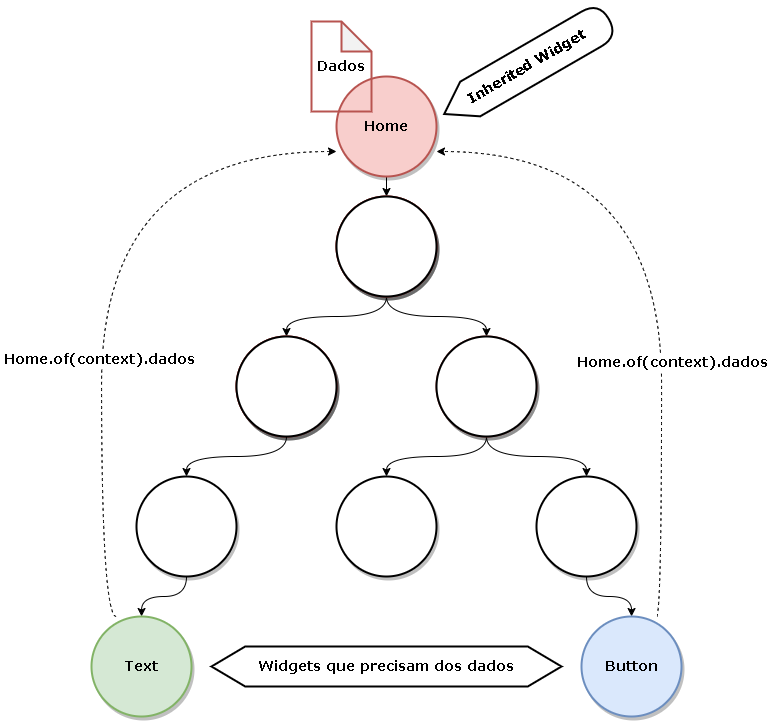
\includegraphics[width=0.8\textwidth]{figuras/cap2/2_2_2_inherited-widget-diagram.png}
  \caption{Exemplo de uma árvore de widgets com InheritedWidget. \protect\cite{Faust2020} \protect\cite{boelens2018}}
  \label{fig:inherited-widget-diagram}
\end{figure}

Neste exemplo, o estado é mantido pelo \textit{widget} nomeado como \textbf{Home} e é acessado pelos \textit{widgets} \textbf{Text} e \textbf{Button} por meio do método estático \textit{Home.of(BuildContext context)} que, por sua vez, busca no contexto dessa sub-árvore, o \textit{widget} mais próximo que seja do exato tipo \textit{Home} e que seja uma extensão concreta da classe InheritedWidget.
% ref: https://api.flutter.dev/flutter/widgets/InheritedWidget-class.html 10/11/2022
% ref: https://api.flutter.dev/flutter/widgets/BuildContext/dependOnInheritedWidgetOfExactType.html 10/11/2022
% \subsection{Principais características}
% A fazer.

\subsection{Diferenças para outras tecnologias}
\label{cap2:Subsec:DiferencasTecnologias}
A fazer.
 % ref: https://hackernoon.com/whats-revolutionary-about-flutter-946915b09514

\subsection{Gerenciamento de estado}
\label{cap2:Subsec:GerenciamentoEstado}
O gerenciamento de estado no \textit{Flutter} não segue apenas uma arquitetura. Na verdade, o \textit{framework} oferece uma série de opções para que o desenvolvedor possa escolher a que melhor se adapta ao seu projeto \cite{Faust2020}. Algumas das principais opções são: \textit{InheritedWidget}, \textit{Provider}, \textit{MobX} \textit{BLoC} e \textit{Redux}. Cada uma dessas opções possui suas vantagens e desvantagens, sendo que algumas são mais adequadas para projetos pequenos e outras para projetos maiores. Anteriormente, descreveu-se o funcionamento do \textit{InheritedWidget} e, mais a frente, serão apresentadas as principais características sobre o \textit{Provider} e o \textit{MobX}.
% ref: https://docs.flutter.dev/development/data-and-backend/state-mgmt/options 10/11/2022

Antes, porém, é importante destacar que o \textit{Flutter}, diferente de outros \textit{framework}s de desenvolvimento de aplicações \textit{mobile}, como o \textit{Android SDK} e o \textit{iOS UIKit}, não segue uma perspectiva imperativa, onde é possível alterar o estado de um \textit{widget} diretamente. Em vez disso, o \textit{Flutter} segue uma perspectiva declarativa, onde a interface do usuário é alterado através de uma função que retorna um novo \textit{widget}. Isso significa que, ao alterar o estado de um \textit{widget}, o \textit{framework} irá reconstruir esse \textit{widget}, mesmo que isso aconteça a cada novo \textit{frame} da aplicação. O processo pode ser custoso, mas o \textit{Flutter} é rápido o suficiente para isso e existem vantagens associadas, principalmente o benefício de determinar como a interface deve ser construída dado um estado específico e mantê-la assim até que haja a necessidade de uma reconstrução dessa interface.
% ref: https://docs.flutter.dev/development/data-and-backend/state-mgmt/declarative 10/11/2022

\subsection{\textit{Provider}}
\label{cap2:Subsec:Provider}

\textit{Provider} é um \textit{wrapper}, isto é, um encapsulamento que envolve o \textit{InheritedWidget} com o objetivo de simplificar seu uso e, com isso, facilitar o gerenciamento de estados em aplicações \textit{Flutter}.
% ref: https://pub.dev/packages/provider 10/11/2022

Ao utilizar o \textit{Provider}, pode-se encapsular o estado em uma nova classe que herda de \textit{ChangeNotifier} ou se mistura a ela com o uso da palavra reservada \textit{with}, do Dart. Dessa forma, essa classe ganha a capacidade de notificar os \textit{widgets} que se subscrevem a ela quando o estado é alterado. Para isso, basta utilizar o método \textit{notifyListeners()} em métodos que alteram esse estado.
% ref: https://docs.flutter.dev/development/data-and-backend/state-mgmt/simple
% ref: https://www.youtube.com/watch?v=d_m5csmrf7I 10/11/2022

Para injetar o estado aos widgets que tem interesse nele, utiliza-se o \textit{ChangeNotifierProvider}. Esse \textit{widget} é colocado acima dos widgets que devem receber a instância do \textit{ChangeNotifier}. Por fim, para consumir o estado e responder às suas mudanças, utiliza-se um \textit{widget} chamado \textit{Consumer}, o qual é normalmente colocado ao redor do \textit{widget} que deve ser atualizado quando o estado é alterado. Também pode-se utilizar o método \textit{Provider.of(context)} para obter o estado ou alterá-lo.
% ref: https://docs.flutter.dev/development/data-and-backend/state-mgmt/simple
% ref: https://www.youtube.com/watch?v=d_m5csmrf7I 10/11/2022

\subsection{\textit{MobX}}
\label{cap2:Subsec:MobX}
% [A revisar]
\textit{MobX} é uma biblioteca para gerenciamento de estado baseado em reatividade \cite{mobx-package}. A reatividade, nesse contexto, é um conceito que permite que o estado de um \textit{widget} mude automaticamente quando uma ação é realizada em outro local, como por exemplo, um outro \textit{widget}. Para isso, utiliza-se a ideia de observabilidade a partir do \textit{widget} que depende do estado a ser observado e, assim que este é alterado, o \textit{widget} é notificado e reconstruído. Esse ciclo pode ser demonstrado na imagem \ref{fig:mobx-cycle}.


\begin{figure}[!ht]
  \centering
  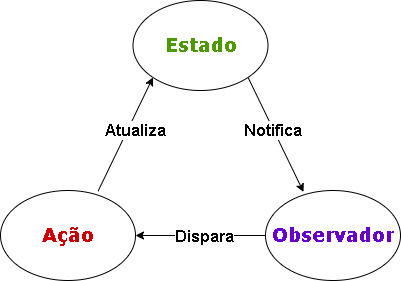
\includegraphics[width=0.6\textwidth]{figuras/cap2/2_2_6_mobx-cycle.png}
  \caption{Ciclo básico do gerenciamento de estado com o MobX \protect\cite{mobx-package} \protect\cite{podila18mobx}}
  \label{fig:mobx-cycle}
\end{figure}


A \textbf{ação} é responsável por gerar mudança no estado da aplicação. Ela pode ser disparada por uma interação do usuário com algum \textit{widget}, como um botão, assim como pode ser resposta a um efeito colateral causado por uma outra ação anterior a esta e que gerou uma mudança de estado anterior, a qual foi consumida por um observador.

O \textbf{observador}, por sua vez, pode ser um \textit{widget}, que apresentará uma mudança visual ao usuário ou uma função responsável por lidar com a mutação desse estado, mas sem que haja, necessariamente, uma reconstrução da interface.

E, por fim, o \textbf{estado} é o valor que será observado e que, quando alterado, notificará os observadores. Esse estado pode ser uma variável, um objeto ou uma lista de objetos, por exemplo.

A notificação realizada pelo estado pode ocasionar efeitos colaterais em outros observadores, que por sua vez, podem disparar novas ações, gerando um ciclo de reatividade. A imagem \ref{fig:mobx-details} apresenta uma representação mais detalhada do ciclo com o \textit{MobX}.

\begin{figure}[!ht]
  \centering
  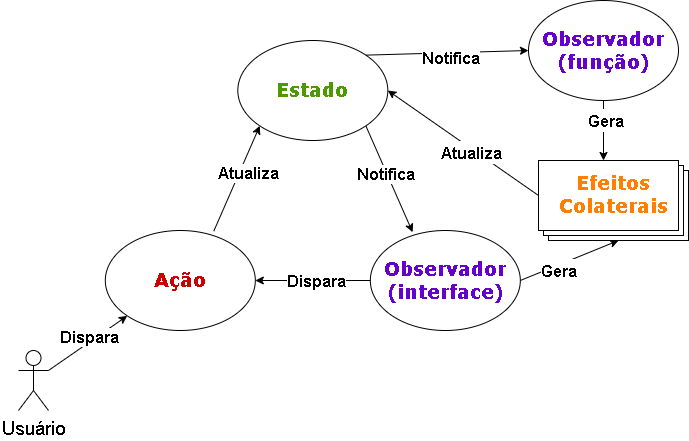
\includegraphics[width=0.9\textwidth]{figuras/cap2/2_2_6_mobx-details.png}
  \caption{Ciclo detalhado do gerenciamento de estado com o MobX \protect\cite{mobx-package} \protect\cite{podila18mobx}}
  \label{fig:mobx-details}
\end{figure}

% [A analisar] [A fazer] Exemplo genérico da implementação do MobX.


% \section{Programação Orientada a Objetos}
% A fazer.

\section{Persistência de Dados}
\label{cap2:Sec:PersistenciaDados}
% [A revisar]
A persistência de dados no contexto do Flutter é o processo de armazenamento em disco das informações relativas à aplicação ou ao seu usuário.
A persistência de dados em um aplicativo móvel permite que o usuário possa acessar as informações mesmo quando não estiver conectado à internet ou mesmo quando o aplicativo estiver fechado. As principais formas de armazenamento de dados em uma aplicação Flutter são: salvamento em \textit{Shared Preferences}, leitura e escrita de arquivos e salvamento em banco de dados \textit{SQLite} \cite{persistence}.
% ref: https://docs.flutter.dev/cookbook#persistence 12/11/2022

A forma como as informações são salvas dependem da quantidade, complexidade e finalidade delas. Para pequenos conjunto de dados, o salvamento em chave-valor, utilizando o \textit{Shared Preferences}, é uma boa opção \cite{shared_preferences}. Já para arquivos de texto, como por exemplo, um arquivo \textit{JSON}, o salvamento em disco é uma boa opção, pois permite a leitura e escrita de dados de forma mais abrangente em relação ao tipo de arquivo salvo e sua utilidade posterior \cite{reading_writing_files}. Por fim, para grandes conjuntos de dados, como por exemplo, uma lista de contatos, o \textit{SQLite} é preferível, pois ele é uma biblioteca que implementa o mecanismo de um banco de dados relacional \cite{sqlite-org} que permite a criação de tabelas e a manipulação de dados de forma simples e rápida \cite{sqlite-flutter} \cite{sqlite_features}.

No contexto da aplicação, a quantidade de dados pode ser consideravelmente grande e estão bastante relacionados entre si, como descrito na \ref{cap4:SubSec:DiagramaClasses}. Por conta disso, a estratégia utilizada é a de salvar os dados em banco relacional, utilizando o \textit{SQLite}.

\subsection{\textit{Banco de Dados SQLite}}
\label{cap2:SubSec:BancoSQLite}
Um banco de dados pode ser entendido como um conjunto organizado e integrado de dados ou informações que atendem a um conjunto de usuários \cite{heuser09banco} \cite{oracle}. Em geral, os bancos de dados tem o objetivo de armazenar dados de vários sistemas e/ou usuários diferentes e, por conta disso, utilizam-se de sistemas de gerenciamento de banco de dados (SGBD) modularizados \cite{heuser09banco} que, em alguns casos, exigem um servidor a parte para realizar os processos que recebem em uma arquitetura conhecida como cliente/servidor \cite{sqlitetutorial_net}.

Para esse tipo de banco de dados, o foco está mais atrelado à escalabilidade e concorrência de dados, visto que inúmeros novos sistemas podem ser acoplados ao banco de dados pré-existente. No caso do \textit{SQLite}, o foco está mais voltado para a economia, eficiência e simplicidade, ao passo em que ele atenderá a um único sistema ou aplicação que, nesse caso, se trata do dispositivo móvel e dos poucos usuários (em geral, apenas um), que o utilizarão \cite{sqlite_use}.

\subsection{Modelagem do banco de dados}
\label{cap2:SubSec:ModelagemBD}

A modelagem dos dados que serão salvos em um banco fornece uma representação abstrata da estrutura das informações que estarão contidas ali. Essa modelagem normalmente segue dois níveis de abstração diferentes que são criados de acordo com a finalidade e com o momento de desenvolvimento do projeto. O \textbf{modelo conceitual} normalmente possui informações menos detalhadas, mas que passam uma ideia geral da estrutura que será criada no banco de dados e os tipos de informação que estarão presente. Posteriormente, cria-se um \textbf{modelo lógico}, o qual já depende do SGBD utilizado e possui mais detalhes sobre os tipos de informações que possui e a forma como elas serão gravadas. \cite{heuser09banco}.

A seguir, na figura \ref{fig:diagrama_er}, é apresentada um exemplo de modelagem conceitual do banco de dados, utilizando-se uma parte simplificada da aplicação e, na figura \ref{fig:diagrama_logico}, a modelagem lógica para a mesma parte da aplicação.

\begin{figure}[!ht]
    \centering
    
\includegraphics[width=0.8\textwidth]{figuras/cap2/2_3_2_diagrama-er.png}
    \caption{Modelagem conceitual de parte do banco de dados}
    \label{fig:diagrama_er}
\end{figure}

\begin{figure}[!ht]
    \centering
    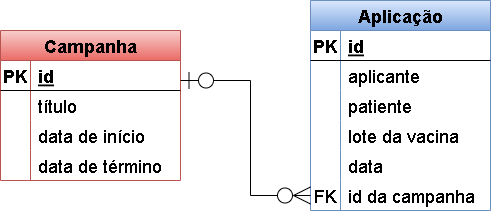
\includegraphics[width=0.8\textwidth]{figuras/cap2/2_3_2_diagrama-logico.png}
    \caption{Modelagem lógico de parte do banco de dados}
    \label{fig:diagrama_logico}
\end{figure}

Observa-se que a notação utilizada no relacionamento entre as entidades 'Campanha' e 'Aplicação', para ambas as modelagens, segue o padrão conhecido como notação Engenharia de Informações. Nesse tipo de notação, a relação é demonstrada por uma linha e a cardinalidade é representada pelos símbolos nas extremidades dessa linha, ligados à entidade. Ademais, a denominação do relacionamento é dado pelas frases verbais que estão presentes na relação  \cite{heuser09banco}. No caso do relacionamento 'Campanha' e 'Aplicação', ele é representado por 'realiza' e 'é realizada em'.

% ref: [cap 1]
% ref: [cap 5: intro] do livro do heuser


%ref: Projeto de Banco de Dados - C. A. Heuser: Capítulo 1: Seção 1.1.1:  A solução para evitar a redundância não controlada de informações é o compartilhamento de dados. Nesta forma de processamento, cada informação é armazenada uma única vez, sendo acessada pelos vários sistemas que dela necessitam (Figura 1.2). \textit{Ao conjunto de arquivos integrados que atendem a um conjunto de sistemas dá-se o nome de banco de dados (BD)}.

% \section{Arquitetura de Sistemas}
% A fazer.

% \section{Princípios SOLID}

% \subsection{Single Responsibility Principle}
% A fazer.

% \subsection{Open/Closed Principle}
% A fazer.

% \subsection{Liskov Substitution Principle}
% A fazer.

% \subsection{Interface Segregation Principle}
% A fazer.  

% \subsection{Dependency Inversion Principle}
% A fazer.

